\chapter{Introduction to the UR3}
\section{Important}
Read the entire lab before starting and especially the ``Grading" section so you know what needs to be accomplished before finishing the lab.
\section{Objectives}
The purpose of this lab is to familiarize you with the UR3 robot arm and its industrial programming interface called the teach pendant.\
In this lab, you will:
\begin{itemize}
\item Learn how to turn on and activate the UR3, and work with the teach pendant to create a simple program for the UR3
\item Use the teach pendant to turn on and off the suction cup gripper and use the gripper in a program
\item Move three stacked blocks from one position to another position using the rules specified for the Tower of Hanoi puzzle.  Blocks should be aligned on top
of each other.
\item Use high level ``\textbf{Move}" commands to move the UR3's Tool Center Point in linear and circular motions
\item Time permitting play with other functionality of the teach pendant.
\end{itemize}

\section{References}
\begin{itemize}
\item UR3 Owner's Manual:

\url{https://www.universal-robots.com/download/?option=52870#section52851}
\item UR3 Software Manual:

\url{https://www.universal-robots.com/download/?option=53077#section53064}
\item Universal Robots Academy

\url{https://www.universal-robots.com/academy/}

\item Since this is a robotics lab and not a course in computer science or discrete math, feel free to Google for solutions to the Tower of Hanoi\
problem.\footnote{\url{http://www.cut-the-knot.org/recurrence/hanoi.shtml} (an active site, as of this writing.)} You are \textbf{NOT} required to implement\
a recursive solution.
\end{itemize}

\section{Pre-Lab}
Before you come to lab it is very important that you go through the training videos found at Universal Robots website\
\url{https://www.universal-robots.com/academy/}.  These training sessions get into some areas that we will not be using in this\ 
class (for example you will not be changing safety settings), but go through all of the assignments as they will help you\ 
get familiar with the UR3 and its teach pendant.  You also may want to reference these sessions when you are in lab.

\section{Task}
The goal is to move a ``tower'' of three blocks from one of three locations on the table to another.  An example is shown in \figref{towers1}.  The\
blocks are numbered with block 1 on the top and block 3 on the bottom.  When moving the stack, two rules must be obeyed:
\begin{enumerate}
\item Blocks may touch the table in only three locations (the three ``towers'').  
\item You may not place a block on top of a lower-numbered block, as illustrated in \figref{legal1}.
\end{enumerate}

\begin{figure}
	\centering
		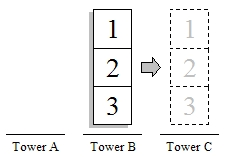
\includegraphics[scale=0.65]{image/lab1_towers.jpg}
	\caption{\figlbl{towers1} Example start and finish tower locations.}
\end{figure}

\begin{figure}
	\centering
		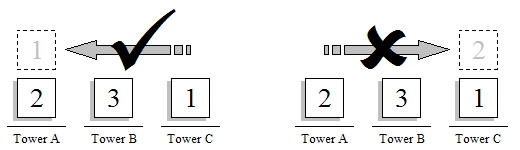
\includegraphics[scale=0.75]{image/lab1_legal.jpg}
	\caption{\figlbl{legal1} Examples of a legal and an illegal move.}
\end{figure}

\section{Procedure}
\begin{enumerate}
\item The Pre-Lab asked you to go through the basic UR3 training at Universal Robots website.  This training should have shown you how to make\ 
simple programs to move the UR3.  Initially your TA will demonstrate how to turn on and enable the UR3 as well as how to use the emergency stop\ 
button.  Then use this lab time to familiarize yourself with the UR3 robot.  First play around with simple programs that move the robot between a\ 
number of points.  
\item To turn on the suction for the suction cup gripper, \textbf{Digital output 0} needs to be set high.  Set low to turn off the suction.  Also \textbf{Digital\ 
input 0} indicates if the suction cup is gripping something.  It will return 1 if it is gripping an object and 0 if not.  Modify your above program\ 
(or make a new one) to add activating on and off the suction cup gripper.  
\item Choose the three spots on the robot's table where blocks can be placed when solving the Tower of Hanoi problem.
\item Use the provided colored tape to mark the three possible tower bases.  You should initial your markers so you can distinguish your\
tower bases from the ones used by teams in other lab sections.
\item Choose a starting position and ending position for the tower of three blocks.  Future note: In Lab 2 the user will enter the start and stop positions.

\item So you will need to use the suction cup gripper's feedback that indicates\ 
whether an object is being gripped or not.  Then with some ``\textbf{If}" instructions complete this task such that the user can put the two blocks in any of the\
three starting positions.  When you are finished, you will demo your program to your TA showning that your program works when two blocks are placed and aligned in the\
three different configurations and also does not have a problem if only one block or even no blocks are placed at their starting positions.  
Tips for creating this program:
\begin{itemize}
\item To turn on the suction cup, use the \textbf{Set} command and select \textbf{Digital Output 0} and turn it on or true.  Set it to off or false to turn off the suction.  
\item \textbf{Digital Input 0} indicates if something has been gripped by the suction cup.  Go to the \textbf{I/O} tab and turn on and off \textbf{Digital Output 0} and check which\
state of Digital Input 0 indicates gripped and upgripped.  
\item In the Structure tab under Advanced besides ``\textbf{If ... else}", you may also want to use the Assignment to create a global worker variable that, for example,\
stores the number of blocks collected.  In addition the \textbf{SubProg} item creates a subroutine that you may call when performing the same steps.  The subroutine's scope\
allows it to see the variables you create with the \textbf{Assignment} item.  
\item You may want to name your \textbf{Waypoints}.  This makes your program easier to read.  In addition if the robot needs to go to the same point multiple times\
in your program you can command it to go to the same waypoint name.  
\item Under the Structure tab you can use the \textbf{Copy} and \textbf{Paste} buttons to copy a line of code and past it in a different subsection of your code.  This cuts down\
on extra typing.  Also note the \textbf{Move} up and down buttons along with the \textbf{Cut} and \textbf{Delete} buttons.  Suppress is like commenting out a line of code.  
\item When you add an ``\textbf{If}" statement and then click on the \textbf{Command} tab, tap in the long white box to pull up the keyboard for entering the if condition.    
\end{itemize} 

\item Using the Teach Pendant create a program that solves the Tower of Hanoi problem.  Instead of using \textbf{MoveJ} moves like in Lab 1, experiment with using\
\textbf{MoveL} and \textbf{MoveP} moves.  \textbf{MoveL} moves the Tool Center Point (TCP) along a straight line, and \textbf{MoveP} is a process move that keeps the TCP moving at a constant\
speed and allows you to move along circular arcs.  Reference these three ``How To" articles from Universal Robots on creating circular arcs:
\begin {itemize}
\item \url{https://www.universal-robots.com/how-tos-and-faqs/how-to/ur-how-tos/circle-using-movec-16270/}
\item \url{https://www.universal-robots.com/how-tos-and-faqs/how-to/ur-how-tos/circular-path-using-movepmovec-15668/}
\item \url{https://www.universal-robots.com/how-tos-and-faqs/how-to/ur-how-tos/circle-with-variable-radius-15367/}
\end {itemize}
\item Demo this working program to your TA.  Your TA may ask you to improve your positioning if the stack does not end up aligned well.
Your program must have at least one obvious linear move and one obvious circular move that completely encircles one of the block positions.
\end{enumerate}
%% Updated by Ben Walt

\section{Report}
Each partner will submit a lab report using the guidelines given in the “ECE 470: How to Write a Lab Report” document.  Please be aware of the following:
\begin{itemize}
	\item Lab reports are due one week after the final session!
	\item Lab reports will be submitted online at \href{https://learn.intl.zju.edu.cn/webapps/login/}{BlackBoard}.
\end{itemize}
Your report should include the following:
\begin{itemize}
	\item Briefly explain the rules of Towers of Hanoi (Introduction/Objective)
	\item Concisely explain your solution (Method)
	\item Discuss your circular movement and how you implemented it (Method)
	\item Note anything you learned about operating the robot (Conclusion)
	\begin{itemize}
		\item How did you keep your block stacks neat?
		\item Observations about \textbf{MoveJ}, \textbf{MoveL}, and \textbf{MoveP}?
	\end{itemize}
	\item Make use of figures and tables as needed to aid in your explanation
	\item Read “ECE 470: How to Write a Lab Report” carefully so you know all the requirements
	  
\end{itemize}

\section{Demo}
Show your TA the program you created.  

\section{Grading}
\begin{itemize}
\item 10 points, completed this section by the end of the two hour lab session.  
\item 70 points, successful demonstration.
\item 20 points, report.
\end{itemize}


% \section{Preparation for Lab 2}
% In Lab 2, we will be moving on to use ROS to control the UR3.  We will use it to solve a modified version of the famous Towers of Hanoi problem.  Some suggested reading:

% \begin{itemize}
% \item Consult Appendix \ref{cprog} of this lab manual for details of ROS and Python functions used to control the UR3.
% \item ``\textit{A Gentle Introduction to ROS}", Chapter 2 and 3. \url{http://coecsl.ece.illinois.edu/ece470/agitr-letter.pdf}
% \begin{itemize}
% \item Chapter 2: 2.4 Packages, 2.5 The Master, 2.6 Nodes, 2.7.2 Messages and message types.
% \item Chapter 3 Writing ROS programs.
% \end{itemize}
% %Doesn't seem to exist anymore - Fall 2020
% %\item A short tutorial for ROS by Hyongju Park. \url{https://sites.google.com/site/ashortrostutorial/}
% \item \url{http://wiki.ros.org/}
% \item Since this is a robotics lab and not a course in computer science or discrete math, feel free to Google for solutions to\
% the Tower of Hanoi problem.\footnote{\url{http://www.cut-the-knot.org/recurrence/hanoi.shtml} (an active site, as of this writing.)} You\
% are not required to implement a recursive solution.

% \end{itemize}